% Template for PLoS
% Version 1.0 January 2009
%
% To compile to pdf, run:
% latex plos.template
% bibtex plos.template
% latex plos.template
% latex plos.template
% dvipdf plos.template

\documentclass[10pt]{article}

% amsmath package, useful for mathematical formulas
\usepackage{amsmath}
% amssymb package, useful for mathematical symbols
\usepackage{amssymb}

% graphicx package, useful for including eps and pdf graphics
% include graphics with the command \includegraphics
\usepackage{graphicx}

% cite package, to clean up citations in the main text. Do not remove.
\usepackage{cite}

\usepackage{color}

% Use doublespacing - comment out for single spacing
%\usepackage{setspace}
%\doublespacing


% Text layout
\topmargin 0.0cm
\oddsidemargin 0.5cm
\evensidemargin 0.5cm
\textwidth 16cm
\textheight 21cm

% Bold the 'Figure #' in the caption and separate it with a period
% Captions will be left justified
\usepackage[labelfont=bf,labelsep=period,justification=raggedright]{caption}

% Use the PLoS provided bibtex style
\bibliographystyle{plos2009}

% Remove brackets from numbering in List of References
\makeatletter
\renewcommand{\@biblabel}[1]{\quad#1.}
\makeatother


% Leave date blank
\date{}

\pagestyle{myheadings}
%% ** EDIT HERE **

%% ** EDIT HERE **
%% PLEASE INCLUDE ALL MACROS BELOW

%% Custom packages that should not violate PLoS author guidelones
\usepackage[greek,english]{babel} % for non-itealic greek letters
\newcommand{\Beta}{\greektext b\latintext}

\newcommand{\TODO}[1]{\textcolor{red}{\textbf{#1}}}

\hyphenation{
microRNA
microRNAs
miRNA
miRNAs
straight-for-ward
}

%% END MACROS SECTION

\begin{document}

% Title must be 150 characters or less
\begin{flushleft}
{\Large
%Methods for integrated data analysis and visualization of cross-platform microarray HA-RAS and CTNNB1 datasets
\textbf{Integrated analysis and visualization of heterogeneous cross-platform microarray datasets}
}
% Insert Author names, affiliations and corresponding author email.
\\
Clemens Wrzodek$^{1,\ast}$,
Elif Unterberger$^{2}$,
Johannes Eichner$^{1}$
Michael Schwarz$^{2}$,
Andreas Zell$^{1}$
\\
\bf{1} Center for Bioinformatics Tuebingen (ZBIT), University of Tuebingen, Sand 1, 72076 T\"ubingen, Germany
\\
\bf{2} Department of Toxicology, Institute of Experimental and Clinical Pharmacology and Toxicology, University of Tuebingen, Wilhelmstrasse 56, 72074 T\"ubingen, Germany
\\
$\ast$ E-mail: clemens.wrzodek@uni-tuebingen.de
\end{flushleft}

% Please keep the abstract between 250 and 300 words
\section*{Abstract}

%TODO: Use words Joint and heterogenous


\TODO{Konzept (technisch): Heute nicht nur mRNA sondern auch viele andere microarrays (miRNA, DNAm, etc.). Daten von den selben samples verf�gbar. Methoden f�r platform�bergreifende datenanalyse und visualisierung sind sehr gefragt.
Konzept (biologisch): Auf Ha-Ras / CTNNB1 eingehen, vor allem platform�bergreifende zusammenh�nge erl�utern und RESULTS dass diese mit den genannten Methoden super analysier/ und visualisierbar sind.}

% Please keep the Author Summary between 150 and 200 words
% Use first person. PLoS ONE authors please skip this step.
% Author Summary not valid for PLoS ONE submissions.
\section*{Author Summary}
\TODO{Eine art subjektive zusammenfassung zu dem artikel schreiben...}


\section*{Introduction}

\TODO{Vor Abgabe suchen und vereinheitlichen von
\begin{itemize}
  \item gene and genome nomenclature
  \item \emph{p}-value
  \item fold-change
  \item Ctnnb1
  \item Ha-ras
  \item up-regulated and down-regulated
  \item BE vs AE (analyses vs. analyzes)
  \item irgendwo erkl�ren dass unsere fold-changes immer log2 based sind!
\end{itemize}
}

In the past, the microarray technology has primarily been used to detect changes in genome-wide gene expression of various biological systems. Usually, a set of biological samples is tested under various experimental and corresponding control conditions. This allows to calculate a relative change in gene expression between treatments and controls, but also between different treatments. Thus, for example, comparisons between differently mutated tumors or animal groups treated with different types of tumor promoters are possible. It has previously been shown that in mice, treatment with the anticonvulsant phenobarbital following a single ip injection of the mutagenic initiator N-diethylnitrosamine (DEN) predominantly leads to liver tumors harboring activating point mutations in the gene encoding the transcription factor \Beta-Catenin, \emph{Ctnnb1} (\TODO{Citation?}). In contrast, tumors isolated from animals treated with DEN only rather carry \emph{Ha-ras}- or \emph{B-raf}-mutations, both of which lead to constant activation of the MAP-kinase signaling pathway \cite{Aydinlik2001}. In the study described by Stahl \emph{et al.}, the microarray approach was used to explore the effect of phenobarbital-treatment on gene expression in mouse liver tumors as compared to non-tumor control tissue \cite{Stahl2005a}.

Today, the application of high-throughput techniques evolved from gene expression to a broad range of other genomic, proteomic and epigenomic features. MicroRNAs (miRNAs) are short non-coding RNAs that regulate gene-expression by potentially binding to complementary mRNA targets \cite{He2004}. MiRNA expression can be measured very similarly to mRNA expression, by defining specific probesets for those RNAs. There are several microarray platforms available today to detect the expression of miRNAs \cite{Hoheisel2006}.

When studying the proteome in context of signaling networks, it is very important to know the phosphorylation state of proteins. In many cases, only phosphorylated proteins become active and propagate a signal, e.g., in a pathway. The expression of basic and phosphorylated proteins can be measured with reverse-phase-protein arrays \cite{Pirnia2009}.

Epigenetic alterations are often detected by measuring DNA methylation of cytosines. It is known that DNA methylation is the only covalent modification of DNA and hypermethylation of cytosines in gene promoters leads to gene silencing of corresponding genes\cite{TheEpigenomicsOfCancer,TheMammalianEpigenome}. The microarray technology has been extended to approaches that tile the promoter regions of defined genes to detect the degree of methylation in those regions \cite{Schumacher2006}.%(TODO: ein wenig erweitern?, auf bisulfite eingehen?)

Using all those microarray technologies (mRNA, miRNA, (phospho-)protein, and DNA methylation), on the same set of biological samples leads to high-dimensional, heterogeneous cross-platform datasets. Figure~1 For most of those individual platforms there are many microarray analysis methods available that go beyond the usual calculation and comparison of fold-changes or other statistical comparisons. But many interesting biological findings are not covered by single platform analysis. The biological system of a cell includes all levels of regulation and omics data expression and therefore, many conclusions can only be drawn when studying multiple genomic layers in parallel.

We here present methods that ease the integrated study of of multiple high-throughput datasets, in which several microarray platforms have been used to investigate various genomic features in the same set of biological samples. The usefulness of those methods is demonstrated by application to a cross-platform dataset of mRNA, miRNA, protein modification, and DNA methylation data, obtained from \emph{Ha-ras}- or \emph{Ctnnb1}-mutated liver tumors in \emph{mus musculus}. These algorithms are going beyond single gene or protein expression analysis (i.e. complementary to locus-specific approaches) and thus into an area of computational biology with a very sparse research density. Interactions detected in heterogeneous datasets have the power to, e.g., reveal novel and very promising biomarker candidates.

\section*{Results and Discussion}

\subsection*{Gene-based integration of heterogeneous datasets}

All proposed methods are validated on a dataset of 19 mouse samples: 10 tumors (3 \emph{Ha-ras}-mutated and not treated with phenobarbital (PB), and 7 \emph{Ctnnb1}-mutated after PB-treatment) and 9 corresponding control tissue samples from the same animals (3 untreated, 6 PB-treated). Messenger RNA, microRNA, DNA methylation and protein modification expression datasets have been measured for all of those samples. We propose to integrate all datasets on gene-level. This is obvious for messenger RNA data, because mapping all probes on genes is a common task. For protein datasets, this is also straightforward, except that different protein modifications should not be mixed. Mapping DNA methylation data on genes requires to introduce a window around the transcription start site (TSS) of each gene. The Nimblegen chip-design provides probes for approximately 8,000 bps downstream and 3,000 bps upstream of each TSS. But including all probes within this window would lead to a huge amount of peaks for one gene, which is difficult to interpret. It has been shown that usually, the proximal promoter region has a stronger effect on a gene's regulation than more distant regions \cite{Cooper2006, Kim2005}. Furthermore, many CpG islands are overlapping the TSS, reaching into the 5' region of a gene \cite{GardinerGarden1987}. And DNA methylation of CpG islands in promoter regions is crucial for the regulation of gene expression \cite{Razin1991}. Putting all together, we decided to assign all probes to a gene that are within -2,000 bps and +500 bps of the TSS.
MicroRNAs infer into gene-regulation by binding to complementary mRNA targets \cite{Bartel2004}. Mapping of microRNA data on genes can be realized by taking the locus of miRNA transcripts or by mapping miRNAs on their corresponding mRNA targets. Both approaches are eligible and have been confirmed by numerous publications \cite{DLK1miRNA,Alexiou2009}. %TODO: Insert Harrys DLK1 paper here if accepted
However, the locus approach is difficult for integrated data analysis, because genes from neighboring loci are not necessarily co-regulated. And integration of different datasets is performed rather on a functional relationship than on a region-based relationship. Therefore, mapping from miRNA to genes is performed by mapping all probes from an miRNA to all genes, whose mRNAs are targets of the miRNA. For this purpose, numerous public databases are available that contain information about miRNAs and corresponding mRNA targets \cite{Alexiou2009}. We worked with a union of three miRNA target databases that only contain experimentally validated tarkets: miRecords v3, miRTarBase v2.4 and TarBase v5.0c \cite{miRecords,miRTarBase,TarBase}.

\subsection*{Methods for integrated data analysis}

Having all platforms integrated, we propose numerous method for integrated representation, visualization and analysis of all platforms.

\subsubsection*{Data pairing}

A first approach that is already suitable for any two datasets is ``data pairing". Data pairing allows viewing two different datasets at once. In the first step, each value from dataset one is mapped on the matching value in dataset two. Then, both values are displayed next to each other in a tabular view. This procedure allows a first glance on integrated data that comes from two platforms. It is especially useful for showing microRNA and mRNA target interactions: the miRNA is shown, together with p-value and fold change on the left hand side, whereas the targeted mRNA is shown, together with p-value and fold change on the right hand side. In the middle between both datasets, the relation is displayed: This includes the source of this target mapping (miRNA target database or prediction algorithm), the confidence of this interaction and the inferred miRNA effect on the mRNA.
%
The InCroMAP application includes all required algorithms to pair any two datasets -� this includes the automated target annotation for miRNA data, the described gene-centering preprocessing steps and the actual creation and rendering of the paired table. An example can be seen in Figure~\ref{fig:2:pairing}.

% PAIRING BILD

Paired analysis of mRNA and miRNA expression data in \emph{Ctnnb1}-mutated tumors revealed miR-495 to be the second most strongly up-regulated miRNA in this tumor type, whereas its expression remains unchanged in \emph{Ha-ras}-mutated tumors. Annotation of experimentally validated targets showed that miR-495 regulates the gene expression of the \emph{Onecut}-transcription factor HNF-6, which itself is down-regulated (see Figure~\ref{fig:2:pairing} and Simion \emph{et al.} \cite{Simion2010}). HNF-6 is known to stimulate the expression of glucose-6-phosphatase (\emph{G6pc}) by binding at its promoter region \cite{Beaudry2006}. The proposed mode of action of miRNA-mediated expression regulation is that an miRNA binds to a complementary mRNA sequence, thus either leading to its degradation or inhibiting its translation at the ribosome. The assumption that miR-495 inhibits the translation of HNF-6 and thus the expression of \emph{G6pc} is a possible explanation for the lack of \emph{G6pc} on protein level in mouse liver tumors \cite{WEBER1955}. The fact that miR-495 is only up-regulated in \emph{Ctnnb1}- but not in \emph{Ha-ras}-mutated tumors whereas both are deficient in G6PC protein indicates that different regulatory mechanisms apply to the two tumor types.

% Vagues gelaber gestrichen.
%In generic, the tabular view resulting from data pairing allows extracting gene markers, which are not visible with a single dataset analysis. Further information can be extracted, by calculating a ``merged fold change" of two different platforms and extract genes that are commonly upregulated, downregulated or show contrary regulations in both datasets. (\TODO{TODO CLEMENS: dies anhand beispielen der obigen figure ausf�hren})


\subsubsection*{Tabular integration of multiple heterogeneous datasets}

Integration of multiple datasets into a tabular view is similar to data pairing, except that more than two datasets are aligned and displayed alongside. One important objective of multiple data integration is showing the relevant information and hiding irrelevant information, as a table might get very big if all information, contained in a paired data table is shown. Thus, one row is created for each gene and one column for each platform. A single summary value of each gene is calculated for each platform and placed in the table. How the summary value is calculated largely depends on the platform and user-preference. There are arguments for taking the probe or peak with maximum differential expression, but still others prefer taking the mean, e.g., for mRNA datasets. The InCroMAP application, in which this integrated analysis method is implemented, allows for selecting the preferred method to calculate the summary value for each platform.

To provide researchers more information than the single summary value of each platform and gene, a special tabular representation is used that allows to collapse and expand rows in a table. Each gene can be expanded to see all platforms, providing data for this gene. Every platforms itself can be further expanded to show more detailed information. This includes, all probes and their expression values for mRNA data and the corresponding protein and protein modification expression for protein datasets. DNA methylation data is showing all peaks in the promoter region of this gene, when expanded and all single probes when the peaks are further expanded. Gene-based expansion of miRNA datasets will show all miRNAs that are targeting this gene, together with probe-level expression values if the miRNAs are further expanded. Figure~\ref{fig:3:multipleIntegration} illustrates an example of this interactive tabular view.

% Vagues gelaber gestrichen.
%With this procedure, researchers can get a first glimpse on matched, heterogeneous datasets. Frequent questions such as: ``If the mRNA fold change is decreasing, is the promoter methylated?" or ``Is this mRNA target of a highly expressed miRNA, if the protein expression is low?" can be answered with a glimpse at the integrated table.

The tabular integration of all platforms reflecting \emph{Ctnnb1}-mutated tumors confirms a strong hypermethylation in the promoter region of \emph{Egfr}, resulting in a mRNA decrease (see Figures~\ref{fig:3:multipleIntegration} and \ref{fig:4:egfrMethylation})\cite{Montero2006}. Down-regulation of \emph{Egfr} is usually a cause for cancer \cite{Zhang2007}. Interestingly, neither the basic protein nor any phosphorylated variant of EGFR shows strong expression changes.


\subsubsection*{Integrated gene set enrichment}

A common data analysis method, especially for mRNA data, is the gene set enrichment analysis. This analysis is performed by creating a gene list (typically by selecting the genes, showing huge differential expression in treatment versus control) and searching for significant enrichments therein. These enrichments can be pathways, gene ontology terms, or genes, regulated by certain transcription factors, or anything else. As a result, researchers can, for example, figure out which pathways are targeted by a certain treatment or compare targeted pathways of genotoxic or non-genotoxic compounds.

% Prozedur-Bild

We propose a cross-platform extension of this procedure for multiple, integrated heterogeneous datasets. The method is depicted in Figure~\ref{fig:5:iEnrichment}. As usually, platform-specific low-level processing and gene-centering procedures are performed for each platform. Each gene is then being assigned a p-value and fold change. Based on these values, a mixed gene pool of significant differentially expressed genes is created, by picking and merging the significantly differentially expressed genes from all platforms. On this mixed gene pool, an enrichment analysis is now performed. As a result, terms (e.g., pathways) are returned that are enriched across all platforms and not only effects of, for example, mRNA or miRNA data analysis. This provides a much broader insight into pathway changes in the organism, upon treatment with a specific compound, than enrichment analysis of a single platform.

Figure~\ref{fig:6:iEnrichmentVsMRNA} shows a comparison between mRNA-only and an integrated gene set enrichment, using mRNA, miRNA, DNA methylation and protein modification data from \emph{Ctnnb1}-mutated tumors. It is clearly visible that the integrated enrichment shows significant changes in many cancer related pathways, whereas the mRNA enrichment shows most significant changes in metabolic pathway maps. Having differentially cancer-related pathways as a results in tumor tissue shows the comprehensiveness of an integrated enrichment, in contrast to platform-specific results, showing in detail which pathways are differentially regulated in this particular platform.


\subsubsection*{Pathway-based visualization of integrated datasets}

Still today, only few visualization techniques are available for integrated datasets. A wide-spread data visualization technique is, creating region-based tracks in a specific file format (common formats are BED or WIG) and using the UCSC genome browser \cite{UCSCBrowser}. This technique is good to get an insight into specific genome regions of interest, but this technique is not specialized on integrated data analysis and fails to give overall impressions. Especially if interesting genes lay on different chromosomes, it is not possible to visualize them together and if researchers do not already have genes of interest, the method fails completely to give a starting point in the visualized data.

Following up the common pathway enrichment analysis, integrated visualization of differentially regulated pathways and measured microarray data gives an overview of how compounds influence certain signaling networks. By changing node colors, shapes, adding new nodes to graphs or adding new labels, much information can be visualized directly in a pathway. Combinations of those possibilities allow visualizing mRNA fold change, miRNA fold change, Protein modification expression data and DNA methylation information directly in a pathway.

%\textbf{Metabolic overview} --
%
To get a comprehensive overview of the regulation of metabolic processes and affected pathways in a microarray dataset, we propose to modify KEGG's ``Metabolic Pathways" map. This pathway visualizes compounds, enzymes and secondary pathways, which are involved in many important metabolic processes in an organism (see Figure~\ref{fig:7:metabolicOverview} and Supplement~\TODO{X}). To visualize specific microarray data and differentially regulated metabolic processes in this pathway, the color of various pathway elements is changed. All downregulated enzymes (depicted as edges between compounds) are colored blue and all upregulated enzymes are colored red. Stronger differential expression is indicated by more saturated colors. With this procedure, the expression of all contained enzymes is visualized, e.g., based on an mRNA dataset. Further, the metabolic overview pathway contains multiple rectangular nodes which are references to secondary metabolic pathways. The color of those referenced pathways can be changed to reflect the p-value of this pathway in an enrichment analyses. In other words, the color of referenced pathways can be changed to a more saturated color if the pathway is significantly differentially regulated in a microarray dataset and to a brighter color if it is less significantly differentially regulated. The resulting picture is an overview which metabolic processes and enzymes are up- or downregulated in any input microarray dataset. See Figure~\ref{fig:7:metabolicOverview} for an example.

% Metabolic overview bild

%\textbf{Pathway-based visualization of cross-platform microarray datasets} --
%
The described method can further be extended to visualize data from multiple platforms in any particular pathway. For most color-based visualizations, we define blue to indicate downregulation and red for upregulation. More saturated colors indicate stronger differential expressions and white is used to visualize no differential expression. Grey is used to show that no data is available from the input dataset.
%
Messenger RNA expression is typically available for the majority of nodes in a pathway. Hence, the background color of every node in a pathway is changed to reflect the mRNA expression change. Protein expression is visualized by adding a small colored box below each node. If multiple measurements are available for differentially modified proteins (e.g., acetylated or phosphorylated isoforms), a separate box is added for each modification. Each box is labeled according to the proteins modification.

Integrating microRNA data into the pathway visualization is more difficult, as pathways usually consist of protein coding genes and compounds. MicroRNAs are not included in pathways and thus, a connection from each miRNA to the nodes in a pathway must be established. As already described, miRNAs are integrated with other platforms by querying miRNA target databases and put the miRNAs in relation to their corresponding targets. The same approach is used for the pathway-based visualization. Each miRNA that has a target within the current pathway is added as small rectangle, which is colored according to miRNA expression. The connection to the target is depicted by a line from the miRNA to the node, corresponding to the target mRNA.

DNA methylation data can be interpreted as a trajectory in a defined window for each gene. This information must be summarized, in order to crete a brief overview for each gene. Since most researchers want to know if a gene is rather hyper- or hypomethylated, we recommend to inspect and visualize the DNA methylation peaks. Visualizing the mean or median is not very informative since small local peaks can already have a strong influence on gene expression. Hence, to get a single summary value for each gene, any peak detection algorithm can be applied to a DNA methylation dataset (see, e.g., the user's guide of Nimblegen's SignalMap software \cite{NimblegenSignalMapUserGuide}) or the peak can be approximated by taking the probe with maximum differential expression on a normalized and smoothed DNA methylation dataset.

\TODO{TODO: Folgende Bloecke ueberarbeiten und etwas results zusammentippen, auf glycolysis fig eingehen, zus�tzlich noch eine fig (wnt/map) mit alle 4 typen.}

The summary value for DNA methylation data is visualized as a black bar that is drawn from the middle to the left side to indicate hypomethylation and from the middle to the right side to indicate hypermethylation. The total size of the bar is proportional to the summary value, i.e., the maximum DNA methylation peak. The aim of this visualization is giving a first hint if a gene promoter is differentially methylated. In the InCroMAP application, the gene can be selected to get a detailed plot of the actual DNA methylation trajectory in the corresponding promoter region (see Figure~\ref{fig:4:egfrMethylation}).

A global overview of metabolic pathways in \emph{Ha-ras}- or \emph{Ctnnb1}-mutated tumors on mRNA level provided a first insight into the profound metabolic changes taking place in the tumors. Integrated enrichment indicated individual pathways with the strongest differential regulation in the respective tumor tissue as compared to normal tissue. The visualizations clearly show characteristic perturbations in the metabolism of \emph{Ctnnb1}-mutated tumors. 

Major transcriptional changes take place in key pathways of energy metabolism, such as glycolysis and gluconeogenesis, the citric acid cycle or the urea cycle. In general, the key enzymes of gluconeogenesis are down-regulated whereas the expression of glucokinase, which catalyzes the first step of glycolysis, is up-regulated. Also, the rate-limiting enzymes of the citric acid cycle are up-regulated. This might indicate that this tumor type uses glucose as fuel rather than synthesizing it \emph{de novo}. Furthermore, the key enzymes of the urea cycle as well as several enzymes involved in amino acid catabolism are characteristically down-regulated in \emph{Ctnnb1}-mutated tumors which is consistent with previous findings \cite{Stahl2005}.



All of the described visualization techniques allow for a joint visualization of mRNA, miRNA, DNA methylation and protein modification data (see Figure~\ref{fig:8:pwVisPlatformsExplanation} for a detailed example of the described visualizations).


%But first, researchers usually start by creating a list of significantly up- or downregulated genes, performing a pathway enrichment analysis and picking significantly enriched and interesting pathways. Our developed algorithm now visualizes the selected pathway, using KEGGtranslator \cite{Wrzodek2011}. In this pathway, a first visualization step is highlighting the genes from the source gene list that lead to the occurrence of this pathway in the enrichment analysis. Going one step further, the mRNA fold change of the source dataset can be visualized as described above.
%This is done by assigning a color to a fold change of zero (e.g. white) a color to a fold change of 4 (e.g. red) and a color to a fold change of -4 (e.g. blue). Now the actual fold change of a gene is visualized by creating a gradient between those colors, matching the actual fold change value. Examples: a gene with a fold change of 1 should be light red and a gene with fold change -1 should be light blue. Genes with fold change of 4 should be deep red and genes with a fold change of 0.1 almost white. This procedure allows at one glance to see the expression fold changes of all genes in a pathway (see Figure 14 for an example).

% ABCD-Erkl�rungsbild \ref{}

% TODO: Von online kopieren...






% You may title this section "Methods" or "Models".
% "Models" is not a valid title for PLoS ONE authors. However, PLoS ONE
% authors may use "Analysis"
\section*{Materials and Methods}

\TODO{TODO: komplette section ueberarbeiten und stark kuerzen!!!}

\subsection*{Samples}

The samples used for the analyses presented here were taken from a previous experiment by Marx-Stoelting \emph{et al.}\cite{MarxStoelting2008}. In brief, male C3H mice received a single dose of DEN and were subsequently kept on a diet containing PB and a PB-free control diet, respectively. \emph{Ctnnb1}-mutated tumors were isolated from the phenobarbital (PB)-treated mice whereas \emph{Ha-ras}-mutated tumors were isolated from the animals which received a PB-free diet. Normal tissue samples were taken from the same livers.

\subsection*{Low-level data processing}

In order to generate processed data from raw data, each data type needs its own low-level data processing procedure. It is important to define standardized procedures here, because the term ``processed data" is not really defined. For example, datasets are sometimes being logarithmized and sometimes not. Another example is the method to calculate p-values or the statistical false discovery rate (FDR) correction afterwards.

As one can see, integrated data analysis does also cover the low-level data processing to generate suitable and comparable high-level data that can be used for the final integrated data analysis methods.

Furthermore, all data must be reduced to a common denominator. The most reasonable common denominator is a gene, thus, all data should be gene-centered after the defined low-level processing steps. The need for this step and our decision to gene-center all datasets is explained in more detail in Section 2.3.

\subsubsection*{Messenger RNA}

EKUT-B received historical and novel mRNA expression data measured by Affymetrix microarrays from the partners EKUT-A, BSP, MUW and UCB in CEL file format. The respective CEL files containing the raw probe intensities were normalized using the Robust Multichip Average (RMA) method and the quality of the experiments was assessed using diverse plots and statistics implemented in the package ``arrayQualityMetrics" for R/Bioconductor [2]. Figure 3 shows a selection of plots generated for Affymetrix gene expression data obtained from MUW. On the basis of extensive quality controls, arrays with limited quality were identified. The corresponding experiments are currently repeated by MUW.

Depending on the study design, a moderated F-statistic (time-series data) or a moderated t-statistic (single time points) was chosen to detect differentially expressed genes (implemention from ``limma" package for R/Bioconductor) [3]. In order to correct for testing multiple genes and to ensure a false discovery rate less than 0.05 the Benjamini-Hochberg method was applied [4]. Additionally, fold change cutoffs of 2 and 0.5 were used to select upregulated and downregulated genes, respectively.

For each treatment and regulation state (i.e. up- or downregulated) a hypergeometric test was performed to identify enriched functional categories and pathways, respectively. Functional categories for characterizing genes with respect to biological process, molecular function and cellular compartment have been chosen according to the Gene Ontology Project (www.geneontology.org). Canonical Pathways were taken from the Biobase database TransPath (www.biobase-international.com), the Ingenuity Knowledge Base (www.ingenuity.com), and the KEGG database (www.genome.jp/kegg). Selected KEGG pathways were overlayed with fold changes, represented by a color gradient, and visualized in interactive graph plots (Figure 8B) to facilitate thorough visual inspection of drug-induced pathway alterations. Furthermore, venn diagrams were generated to illustrate the effects of NGC compounds, differing between cell types or depending on the duration of treatment (Figure 4).

The venn diagrams shown in Figure 4 A2 indicate a CPA-mediated activation of the cell cycle and DNA replication in rodent hepatocytes represented in the deregulated mRNAs. This result, which was exclusively found after in-vivo treatment followed by mRNA expression analysis of hepatocytes isolated from the CPA- and vehicle-treated animals, is consistent with the fact that considerable liver growth was observed for CPA-treated rats. As expected, an upregulation of CYP-dependent metabolism was found, which is most likely due to transcriptional activation by the CAR receptor. This CYP induction could be consistently observed throughout cell types (hepatocytes and mesenchymal cells) and experimental procedures (in-vivo and in-vitro treatment).

\subsubsection*{Micro RNA}

Micro RNA data processing is very similar to messenger RNA data processing. Subsequently we only briefly describe the required steps here. The background-corrected miRNA expression data is logarithmized in the first step. Some miRNAs are not expressed in certain cells and thus, all probes that have a low signal/noise ratio throughout all chips (i.e. the signal is lower than the background noise) are removed. Afterwards, the probes are processed again similar to mRNA data by calculating means, fold changes, p-values and eventually applying statistical correction methods on the calculated p-values.
Integration of micro RNA target databases

Micro RNAs influence the regulation of gene expression in two different ways: either by translational inhibition or target mRNA cleavage. Although there are some evidences for a transcriptional regulation by miRNAs,[5] the common way to interfere into protein biosynthesis is by binding to a messenger RNA and repressing translation or inducing cleavage [6].

Therefore, it is required to know the mRNA targets for a micro RNA to detect the impact of highly up- or downregulated miRNAs and to correlate miRNAs to other datasets. There are many publications, describing miRNA � mRNA interactions[5, 7-16]. Flat data files, summarizing those interactions, can be downloaded from several miRNA target databases. These databases contain experimentally validated miRNA and mRNA target interactions and provide flat-file downloads in different file formats. But still today, these databases only contain subsets of all miRNA � mRNA interactions and hence, many methods to predict mRNA targets of miRNAs have been published[7, 10, 13, 15]. These prediction methods can be used to complete the data available from experimental databases.

EKUT-B has created a comprehensive, integrated miRNA target database that can be used to annotate miRNA datasets with corresponding mRNA targets. This dataset has been created by integrating three experimental miRNA target databases (miRecords v3 [16], miRTarBase v2.4 [12], TarBase v5.0c [14]), removing duplicates and mapping all gene identifiers to common NCBI Gene IDs. This dataset of experimentally validated targets has been completed by adding high-confidence predictions of ElMMo v5 [15], DIANA � microT v4.0 [13] and TargetScan v5.2 [10]. This has proven to be a good combination and integrating more prediction methods might even worsen the resulting miRNA target mapping [7].

Having this target database, gene-centering of miRNA data is performed as follows: first, each miRNA is assigned one value. This is done in the same manner as with mRNA data, e.g. by calculating the mean of all probes for a miRNA. Then, each gene is assigned one or multiple values of microRNAs, regulating the levels of the mRNA encoded by this gene or the translation of this gene�s mRNA.


\subsubsection*{DNA methylation}

Within the MARCAR project, DNA methylation data is measured by Nimblegen promoter tiling arrays, which cover sequence regions of about -8kbps to +3kbps around the transcription start site (TSS) of each gene. This sequence region is tiled with hundreds of probes that are about 50bps in size. The raw probe intensities are processed, as for most microarray platforms, with loess or quantile normalization methods. The resulting probe intensities are smoothed, by incorporating neighboring probe intensities.

The usage of microarray chips to measure DNA methylation is not as easy to interpret as data from other platforms. DNA methylation in mammals affects nearly exclusively the C-5 of cytosines, followed immediately by a guanine. Consequently, probes with similar intensities, but a low CG-content should be treated different than probes with a high CG-content. Furthermore, these values are hard to interpret, because from those signal intensities one cannot read which CGs are methylated and which are not. Thus, methods have been developed that use a fully methylated dataset, in addition to the normal dataset [17]. The fully methylated dataset is obtained by methylation of all cytosines in a DNA and measuring the probe intensities of the same platforms as with the actual data.  The MEDME procedure [17] can then be applied to these datasets. This procedure calculates relative methylation intensities, based on the fully methylated dataset and the CG content of all probes. These relative intensities are then used for further data analysis.

To perform an integrative analysis, it is now required to convert the region-based DNA methylation data to gene-based values. Because DNA methylation is a very region-specific effect, bringing DNA methylation data down to a single value for a gene cannot be done without loss of information. Simple procedures like taking the mean or median of all probes for a gene do not make sense, because local changes in DNA methylation that might have an impact on gene-regulation are not covered then. See for example Figure 5: simply taking the mean of both trajectories results in two very similar values, which do not reflect the actual DNA methylation pattern.

For DNA methylation analyzes, it is not only interesting if the whole promoter is hypo- or hypermethylated, but also if small genomic regions (like CpG islands) are hypo- or hypermethylated. To also catch these local changes, we established a procedure that calculates one value for one gene that tells the researcher if there are local or global methylation changes:

Step 1: Divide the covered sequence region (8kbp downstream and 3kbp upstream of the TSS for Nimblegen chips) into small bins of, e.g. 250bps.

Step 2: Compute p-value pgj based on moderated t-test for each gene g and each bin bj.

Step 3: Compute overall score pg for each gene as follows:

FORMEL FEHLT.

Result: The value pg is very small if the promoter does not show significant DNA methylation changes. A higher value tells the researcher that there are either local significant, or global medium significant methylation changes. A very high value for pg is assigned to promoters with significant global methylation changes.

This procedure does not differentiate between hyper- or hypomethylation and thus, again shows the need for single dataset analyses in addition to integrated data analysis. For an integrated data analysis, the most interesting question is, to detect novel markers that are only visible by having an integrated view on the data. For most of these procedures, a value telling if there are significant methylation changes in a gene-promoter is sufficient. For more detailed analysis, the researcher can then manually take a closer look at the data and see if it is a global or local effect and if the promoter is hypo- or hypermethylated.


\subsubsection*{Protein modification data}

The raw fluorescence intensities measured by Zeptosens Reverse-Phase Protein Arrays (RPPM) were obtained from NMI as a spreadsheet file. At EKUT-B the analytes (i.e. proteins or protein modifications) quantified in diverse biological samples were annotated with UniProt IDs to facilitate the interpretation of the data in the context of signaling pathways. Next, the data was log-transformed and centered around the median intensity values observed for control samples to ease interpretability and obtain a symmetrical scale of protein or protein modification levels. Measurements, for which the background noise (i.e. signal of secondary antibody) was higher than the combined foreground and background signal (i.e. signal of primary and secondary antibody), were treated as missing values and imputed using the k-Nearest-Neighbor (kNN) algorithm.

In order to detect analytes, which are differentially expressed between two sample groups (e.g., treated vs. control samples), a moderated t-test (implementation from ``limma" package for R/Bioconductor) was applied [3]. Subsequently, a correction for multiple hypothesis testing was done using the FDR control method proposed by Benjamini and Hochberg [4]. The results from this statistical analysis were visualized using volcano plots (Figure 6).

The results shown in Figure 6, which shows the volcano plots for NGC-treated rodent hepatocytes, are consistent with findings reported in the literature. For instance, the upregulation of diverse Cytochrome P450 enzymes is a known effect of phenobarbital (PB) treatment, which is mediated via the CAR/PXR receptor. The strong upregulation of Cyclin E2 indicates that PB treatment may also impact on cell cycle regulation.

The analytes were categorized into tissue- and treatment-specific regulation states, respectively, based on significance (p-values from moderated t-statistic) and fold changes. Specifically, regulation states were defined to characterize genes, with regard to the strength (weak, medium, high) and direction (up, down) of differential expression. Expression profiles, composed of the regulation states for each analyte, were clustered using a hierarchical average-linkage approach for the purpose of detecting mechanistic similarities among the treatments (Figure 7). To measure the pairwise similarity of expression profiles (corresponding to rows in Figure 7) an arbitrarily defined scoring matrix was built to score pairs of regulation states, which were in turn summarized across analytes and normalized using a geometric mean.

It becomes obvious from Figure 7 that GCs differ significantly from NGCs in their protein expression profiles. One of the most striking effects observed in Figure 8 is that the Ser235/Ser236-phosphorylated form of S6 Ribosomal protein shows strong upregulation for 100\% (2/2) of the GCs, whereas strong downregulation was observed for 91\% (10/11) of the NGCs, and no differential expression was detected for 100\% (2/2) of the NCs. These results indicate that this protein, which is located in the 40S subunit of the ribosome, and which was reported to impact on cell growth and proliferation [18], is a promising marker for the early detection of nongenotoxic cancerogenicity. In combination with other candidate marker proteins showing class-specific, characteristic expressions patterns (e.g. STAT-3, c-Jun, BAX, etc.), protein signatures facilitating reliable detection of either GC or NGC compounds can be inferred from the data. For this purpose, further investigations are currently pursued by EKUT-B.

Furthermore, EKUT-B identified signaling networks, which are altered in tumor tissue (EKUT-A mouse study) or perturbed after treatment with NGC compounds (BSP rat study), by mapping the analytes to literature-based canonical pathways extracted from the Biobase Knowledge Library (BKL), the Ingenuity Knowledge Base (IKB) and the KEGG database. The impact on canonical pathways was visualized using bar plots showing the fraction of differentially regulated analytes for diverse pathways with potential relevance to the mechanism of NGC compounds (Figure 8).

Figure 8 shows that the differences in the expression profiles of GC and NGC illustrated in Figure 7 come along with considerable differences in the pathways addressed by representative compounds. One of the most obvious findings is that the Wnt pathway, which is known to play a crucial role in the mechanism of NGC compounds, such as PB [19], is exclusively perturbed by treatment with the NGC compounds DHEA and TAA. Among the differentially expressed analytes in the pathway are for instance phosphorylated ?-catenin, phosphorylated GSK3?, and p53 which are known to be key regulators of cell fate.

To obtain a more detailed view of the compound-specific pathway alterations, EKUT-B has implemented a flexible graph viewer which allows visualizing the regulation states of the analytes in the context of signaling networks extracted from KEGG. This is exemplified by Figure 9, which shows the effect of the compound TAA on the Wnt signaling pathway.


\section*{Implementation and availability}
% TODO: erkl�ren von Interactive, Thresholds (max FC) and options (mean, maxFC, median)

% Do NOT remove this, even if you are not including acknowledgments
\section*{Acknowledgments}


%\section*{References}
% The bibtex filename
\bibliography{InCroMAP_methods}

\section*{Figure Legends}

%%%%%%%%%%%%%%%%%%%%%%%%%%%%%%%%%%%%%%
% Introduction - Background picture for all platforms
%%%%%%%%%%%%%%%%%%%%%%%%%%%%%%%%%%%%%%
\begin{figure}[!htb]
  \begin{center}
  %TODO: Convert to TIF (=> look at author guidelines)
  % Source Powerpoint file: "2011-09-20 IntegratedDataAnalysis-Flowchart".
    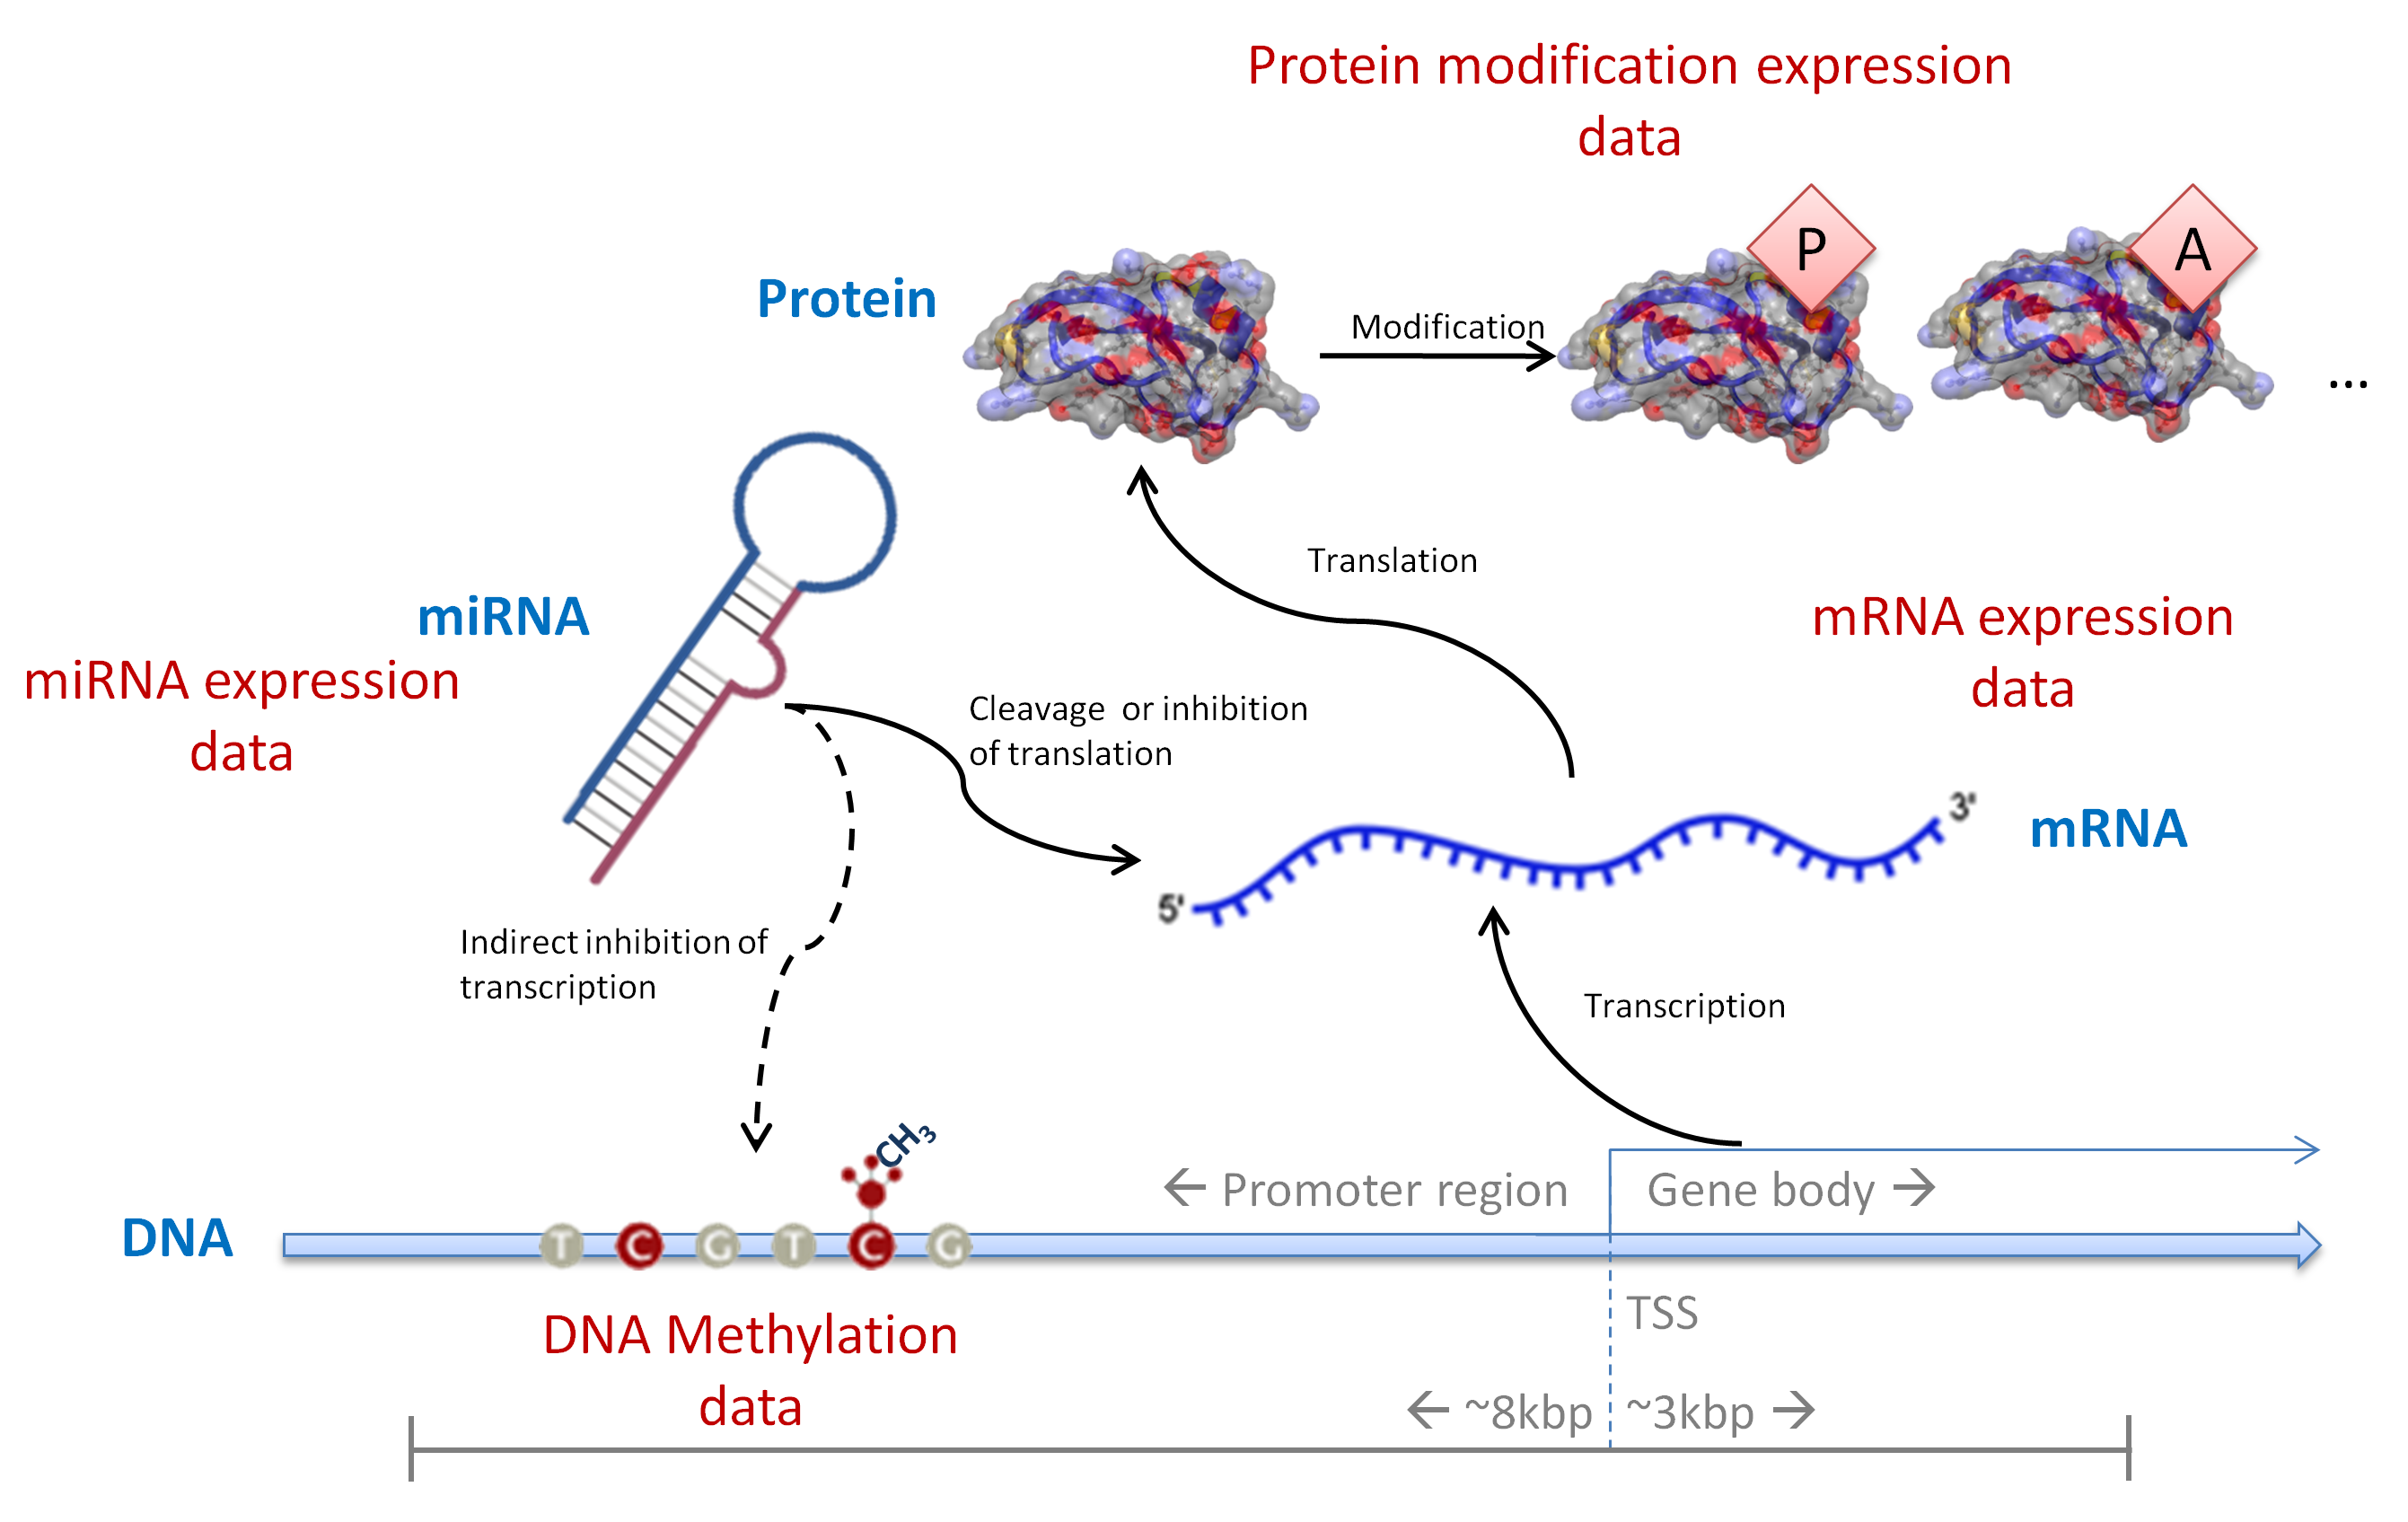
\includegraphics[width=1.0\textwidth]{figures/IntegratedDataAnalysis.png}
  \end{center}

\caption{
{\bf Visualization of diverse microarray platforms that have been employed to perform an integrated data analysis.}
\TODO{1 Caption �berarbeiten, 2 nach M�glichkeit referenz auf farben entfernen, 3 Referenz in Introduction auf Figure einbauen.}
Red fonts describe the actual data types and corresponding platforms. This figure is restricted to genomic interactions relevant for this deliverable. At the bottom of the figure, a DNA sequence is given, for which methylation data is available. This DNA is transcribed to an mRNA. The transcription might be regulated by methylated regions on the gene promoter. Furthermore, miRNAs might inhibit the translation from mRNA to a protein. Both, mRNA and miRNA expression is measured with Affymetrix and Agilent microarrays. In the end, translated proteins might get modified, e.g., by phosphorylation or acetylation. The expression of some basic isoforms and specific modifications is determined, using Zeptosens arrays.
}
\label{fig:1}
\end{figure}


%%%%%%%%%%%%%%%%%%%%%%%%%%%%%%%%%%%%%%
% Data Pairing
%%%%%%%%%%%%%%%%%%%%%%%%%%%%%%%%%%%%%%
\begin{figure}[!htb]
  \begin{center}
  %TODO: Convert to TIF (=> look at author guidelines)
    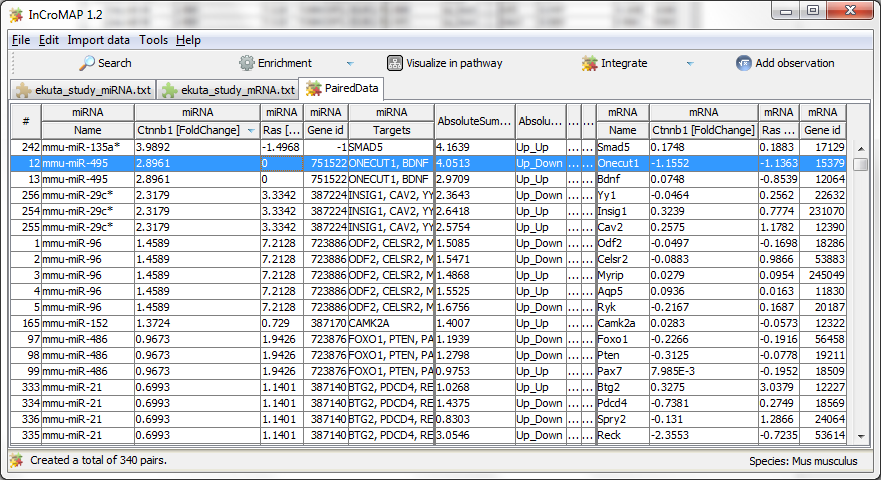
\includegraphics[width=1.0\textwidth]{figures/PairData-Onecut1Story.png}
  \end{center}

\caption{
{\bf Pairing of miRNA (left side) and mRNA (right side) datasets reveals miR-495 as a potential regulator of the HNF-6 coding gene \emph{Onecut1}.}
\TODO{1 Caption �berarbeiten, 2 Ueberlegen ob Ras Expressionswerte ausgeblendet werden sollten und wenn nciht, "in Ctnnb1" in titel.}
}
\label{fig:2:pairing}
\end{figure}


%%%%%%%%%%%%%%%%%%%%%%%%%%%%%%%%%%%%%%
% Multiple Integration
%%%%%%%%%%%%%%%%%%%%%%%%%%%%%%%%%%%%%%
\begin{figure}[!htb]
  \begin{center}
  %TODO: Convert to TIF (=> look at author guidelines)
    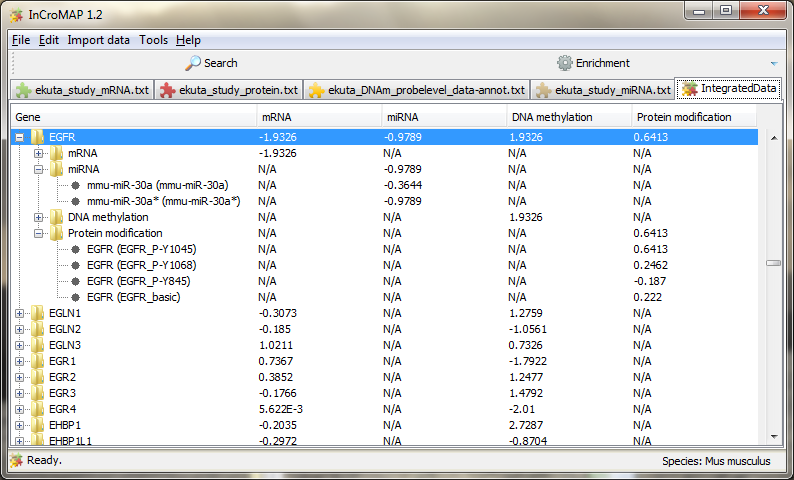
\includegraphics[width=1.0\textwidth]{figures/MultipleIntegrationEGFR.png}
  \end{center}

\caption{
{\bf Multiple integration of four different platforms from \emph{Ctnnb1} mutated tumors shows an mRNA decrease of \emph{Egfr} as a potential effect of DNA methylation increase in the promoter region.}
\TODO{Bildunterschrift}
}
\label{fig:3:multipleIntegration}
\end{figure}


%%%%%%%%%%%%%%%%%%%%%%%%%%%%%%%%%%%%%%
% EGFR Methylation
%%%%%%%%%%%%%%%%%%%%%%%%%%%%%%%%%%%%%%
\begin{figure}[!htb]
  \begin{center}
  %TODO: Convert to TIF (=> look at author guidelines)
    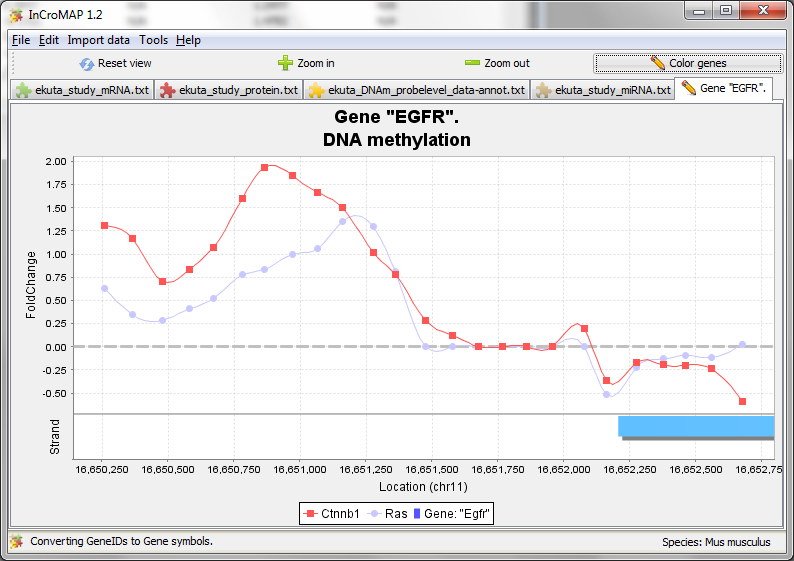
\includegraphics[width=1.0\textwidth]{figures/EGFR_methylation.png}
  \end{center}

\caption{
{\bf DNA methylation in the promoter region of \emph{Egfr} in \emph{Ctnnb1}-mutated tumors.}
\TODO{Bildunterschrift, 2 sagen dass dies auch ein paired ist, da mRNA entsprechend eingef�rbt wurde}
}
\label{fig:4:egfrMethylation}
\end{figure}


%%%%%%%%%%%%%%%%%%%%%%%%%%%%%%%%%%%%%%
% Integrated enrichment
%%%%%%%%%%%%%%%%%%%%%%%%%%%%%%%%%%%%%%
\begin{figure}[!htb]
  \begin{center}
  %TODO: Convert to TIF (=> look at author guidelines)
  % Source Powerpoint file: "2011-09-20 IntegratedDataAnalysis-Flowchart".
    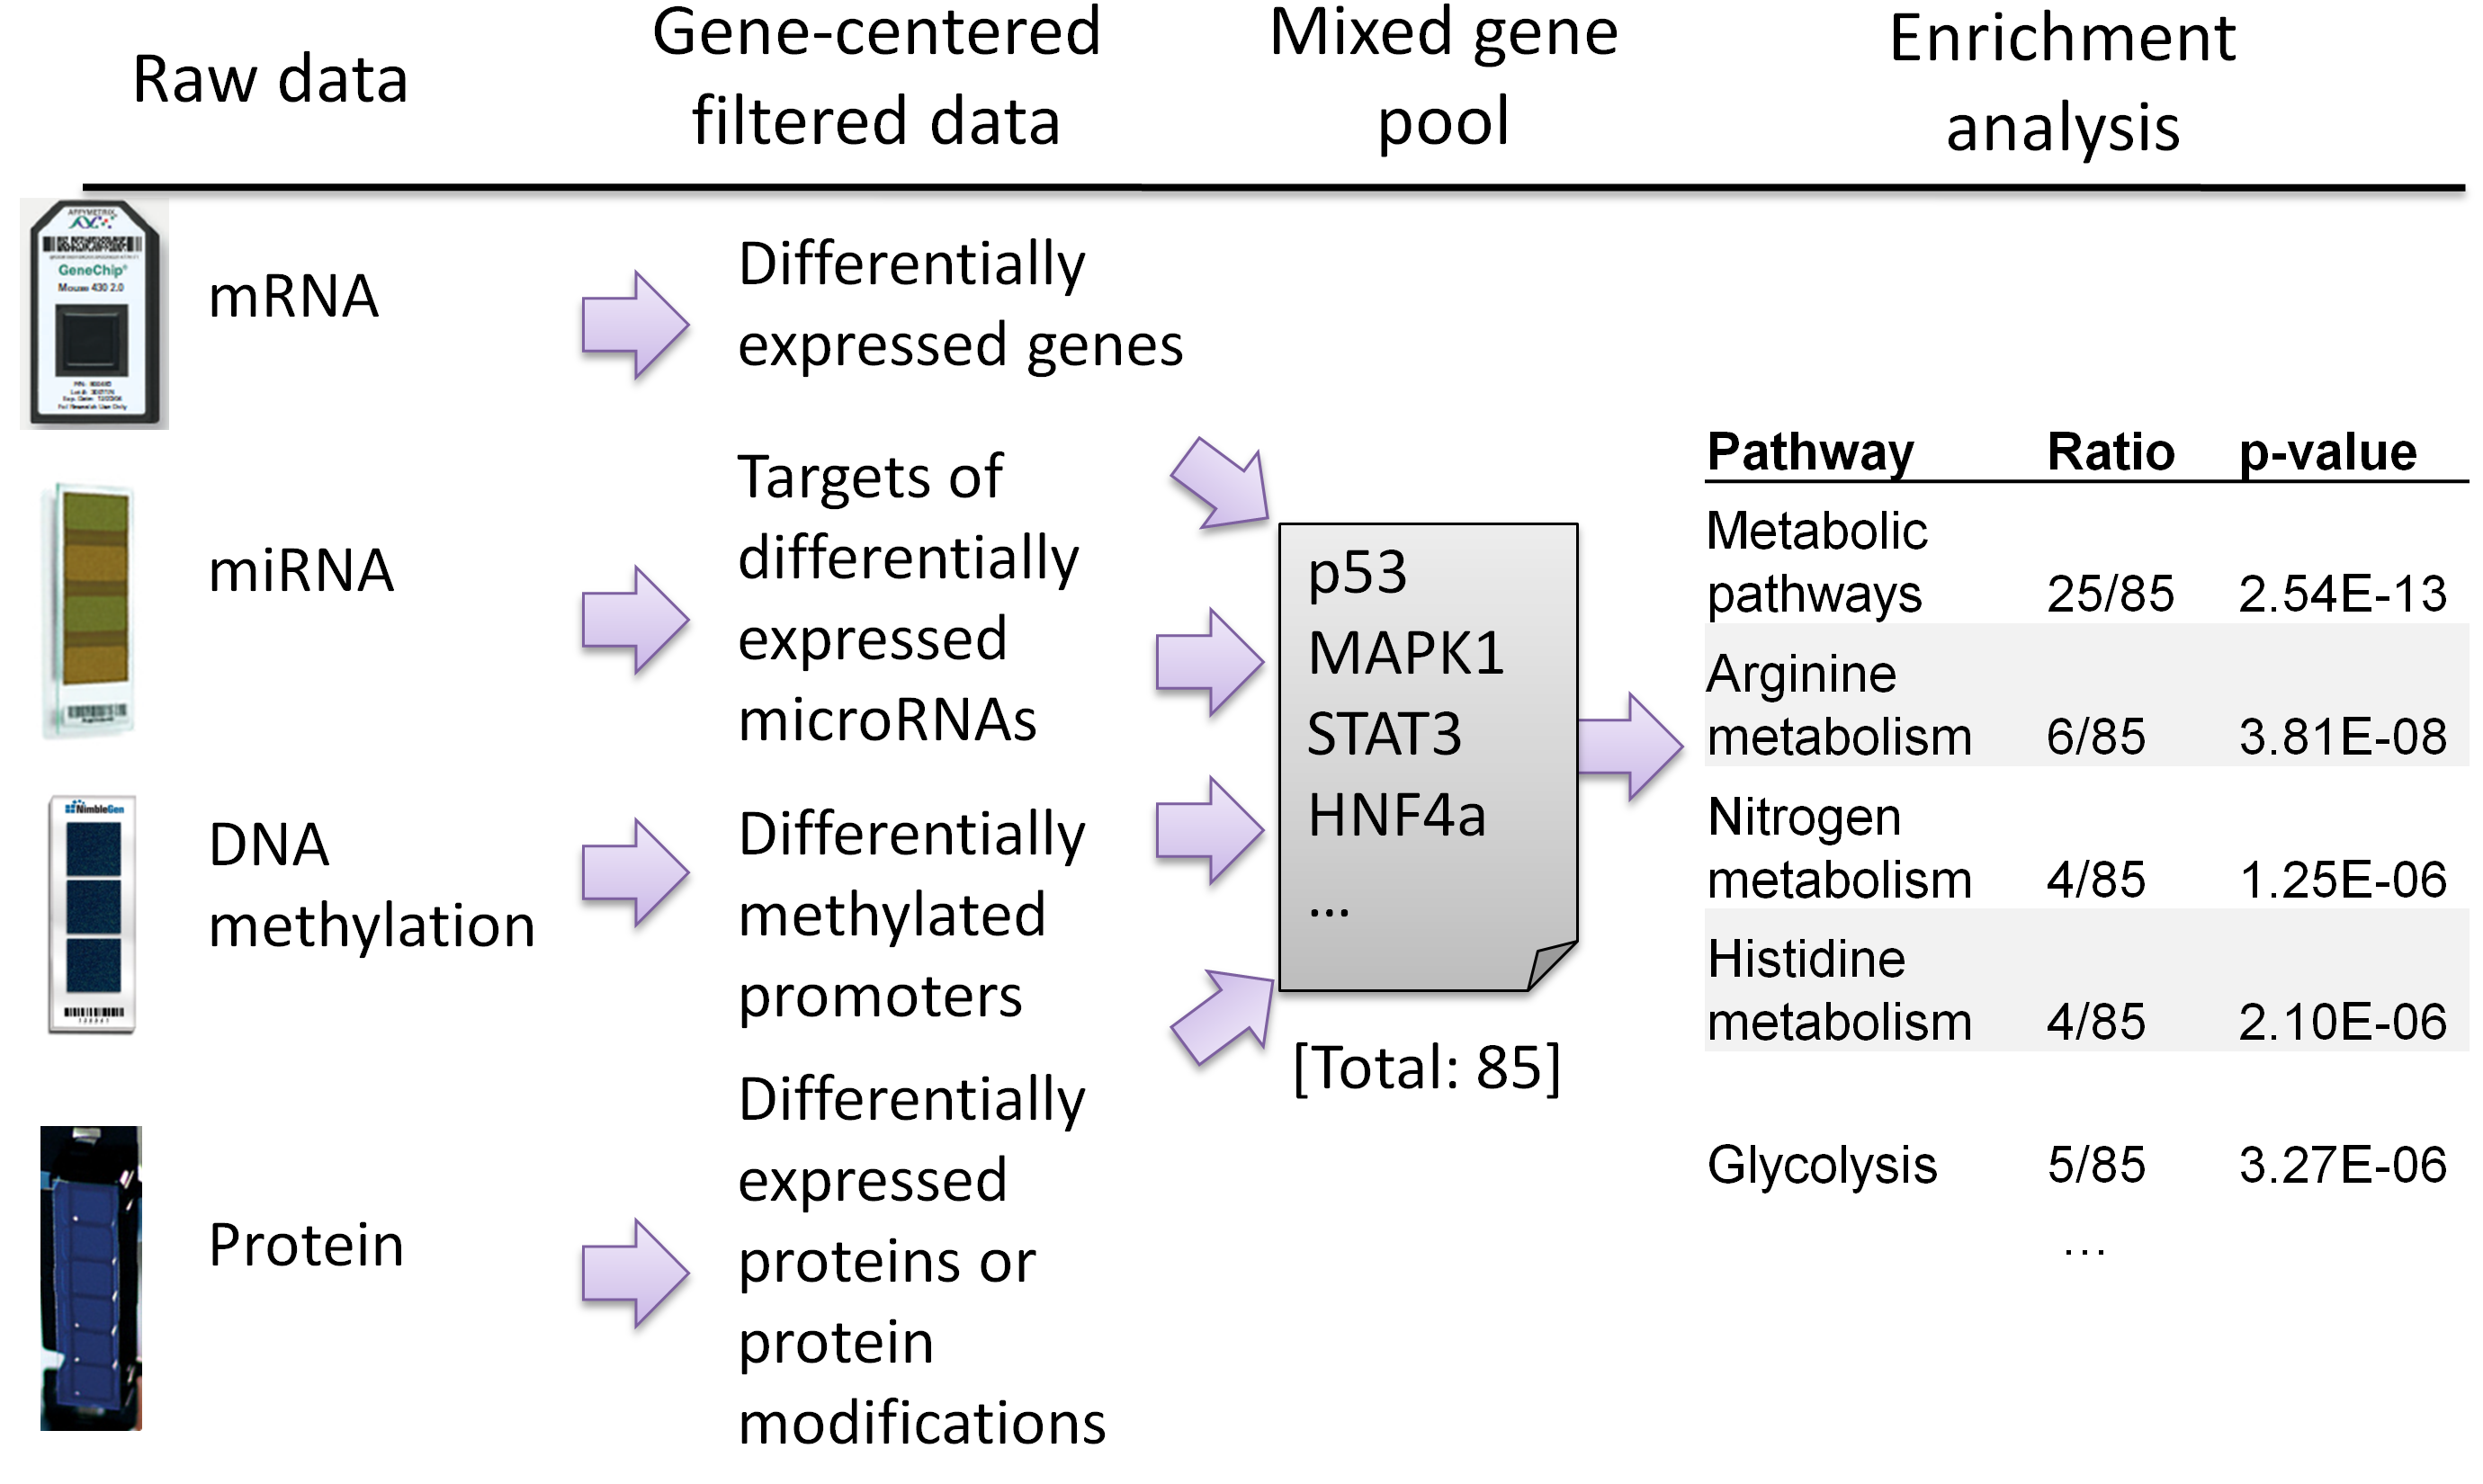
\includegraphics[width=1.0\textwidth]{figures/iEnrichment.png}
  \end{center}

\caption{
{\bf Proposed procedure for a cross-platform gene-set enrichment analysis.}
\TODO{Bildunterschrift, 2 sagen dass 85 usw. examples sind.}
}
\label{fig:5:iEnrichment}
\end{figure}


%%%%%%%%%%%%%%%%%%%%%%%%%%%%%%%%%%%%%%
% Integrated enrichment vs. mRNA enrichment
%%%%%%%%%%%%%%%%%%%%%%%%%%%%%%%%%%%%%%
\begin{figure}[!htb]
  \begin{center}
  %TODO: Convert to TIF (=> look at author guidelines)
    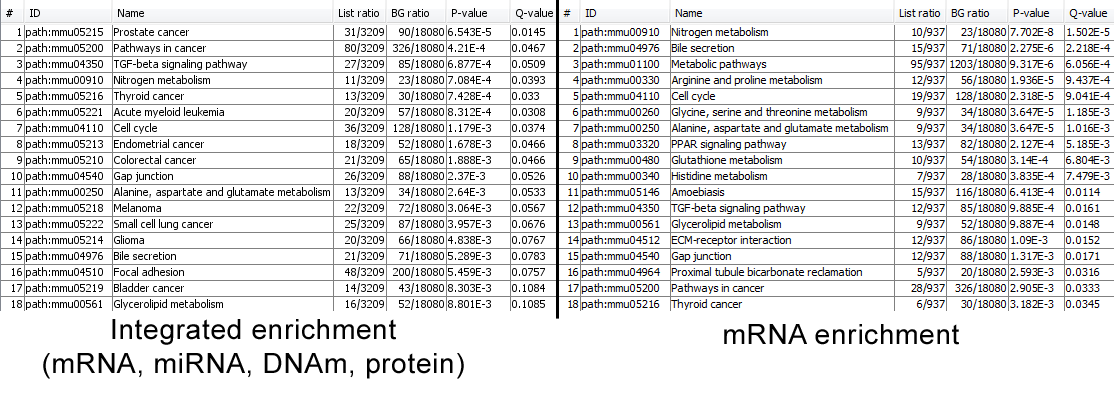
\includegraphics[width=1.0\textwidth]{figures/EnrichmentComparison_cut.png}
  \end{center}

\caption{
{\bf Comparison of an integrated and mRNA enrichment, based on data from Ctnnb1-mutated tumors.}
\TODO{Bildunterschrift, Metabolic vs. Cancer}
}
\label{fig:6:iEnrichmentVsMRNA}
\end{figure}


%%%%%%%%%%%%%%%%%%%%%%%%%%%%%%%%%%%%%%
% Metabolic pathways overview map
%%%%%%%%%%%%%%%%%%%%%%%%%%%%%%%%%%%%%%
\begin{figure}[!htb]
  \begin{center}
  %TODO: Convert to TIF (=> look at author guidelines)
  %TODO: Add full image (+mRNA coloring) as supplementary material
    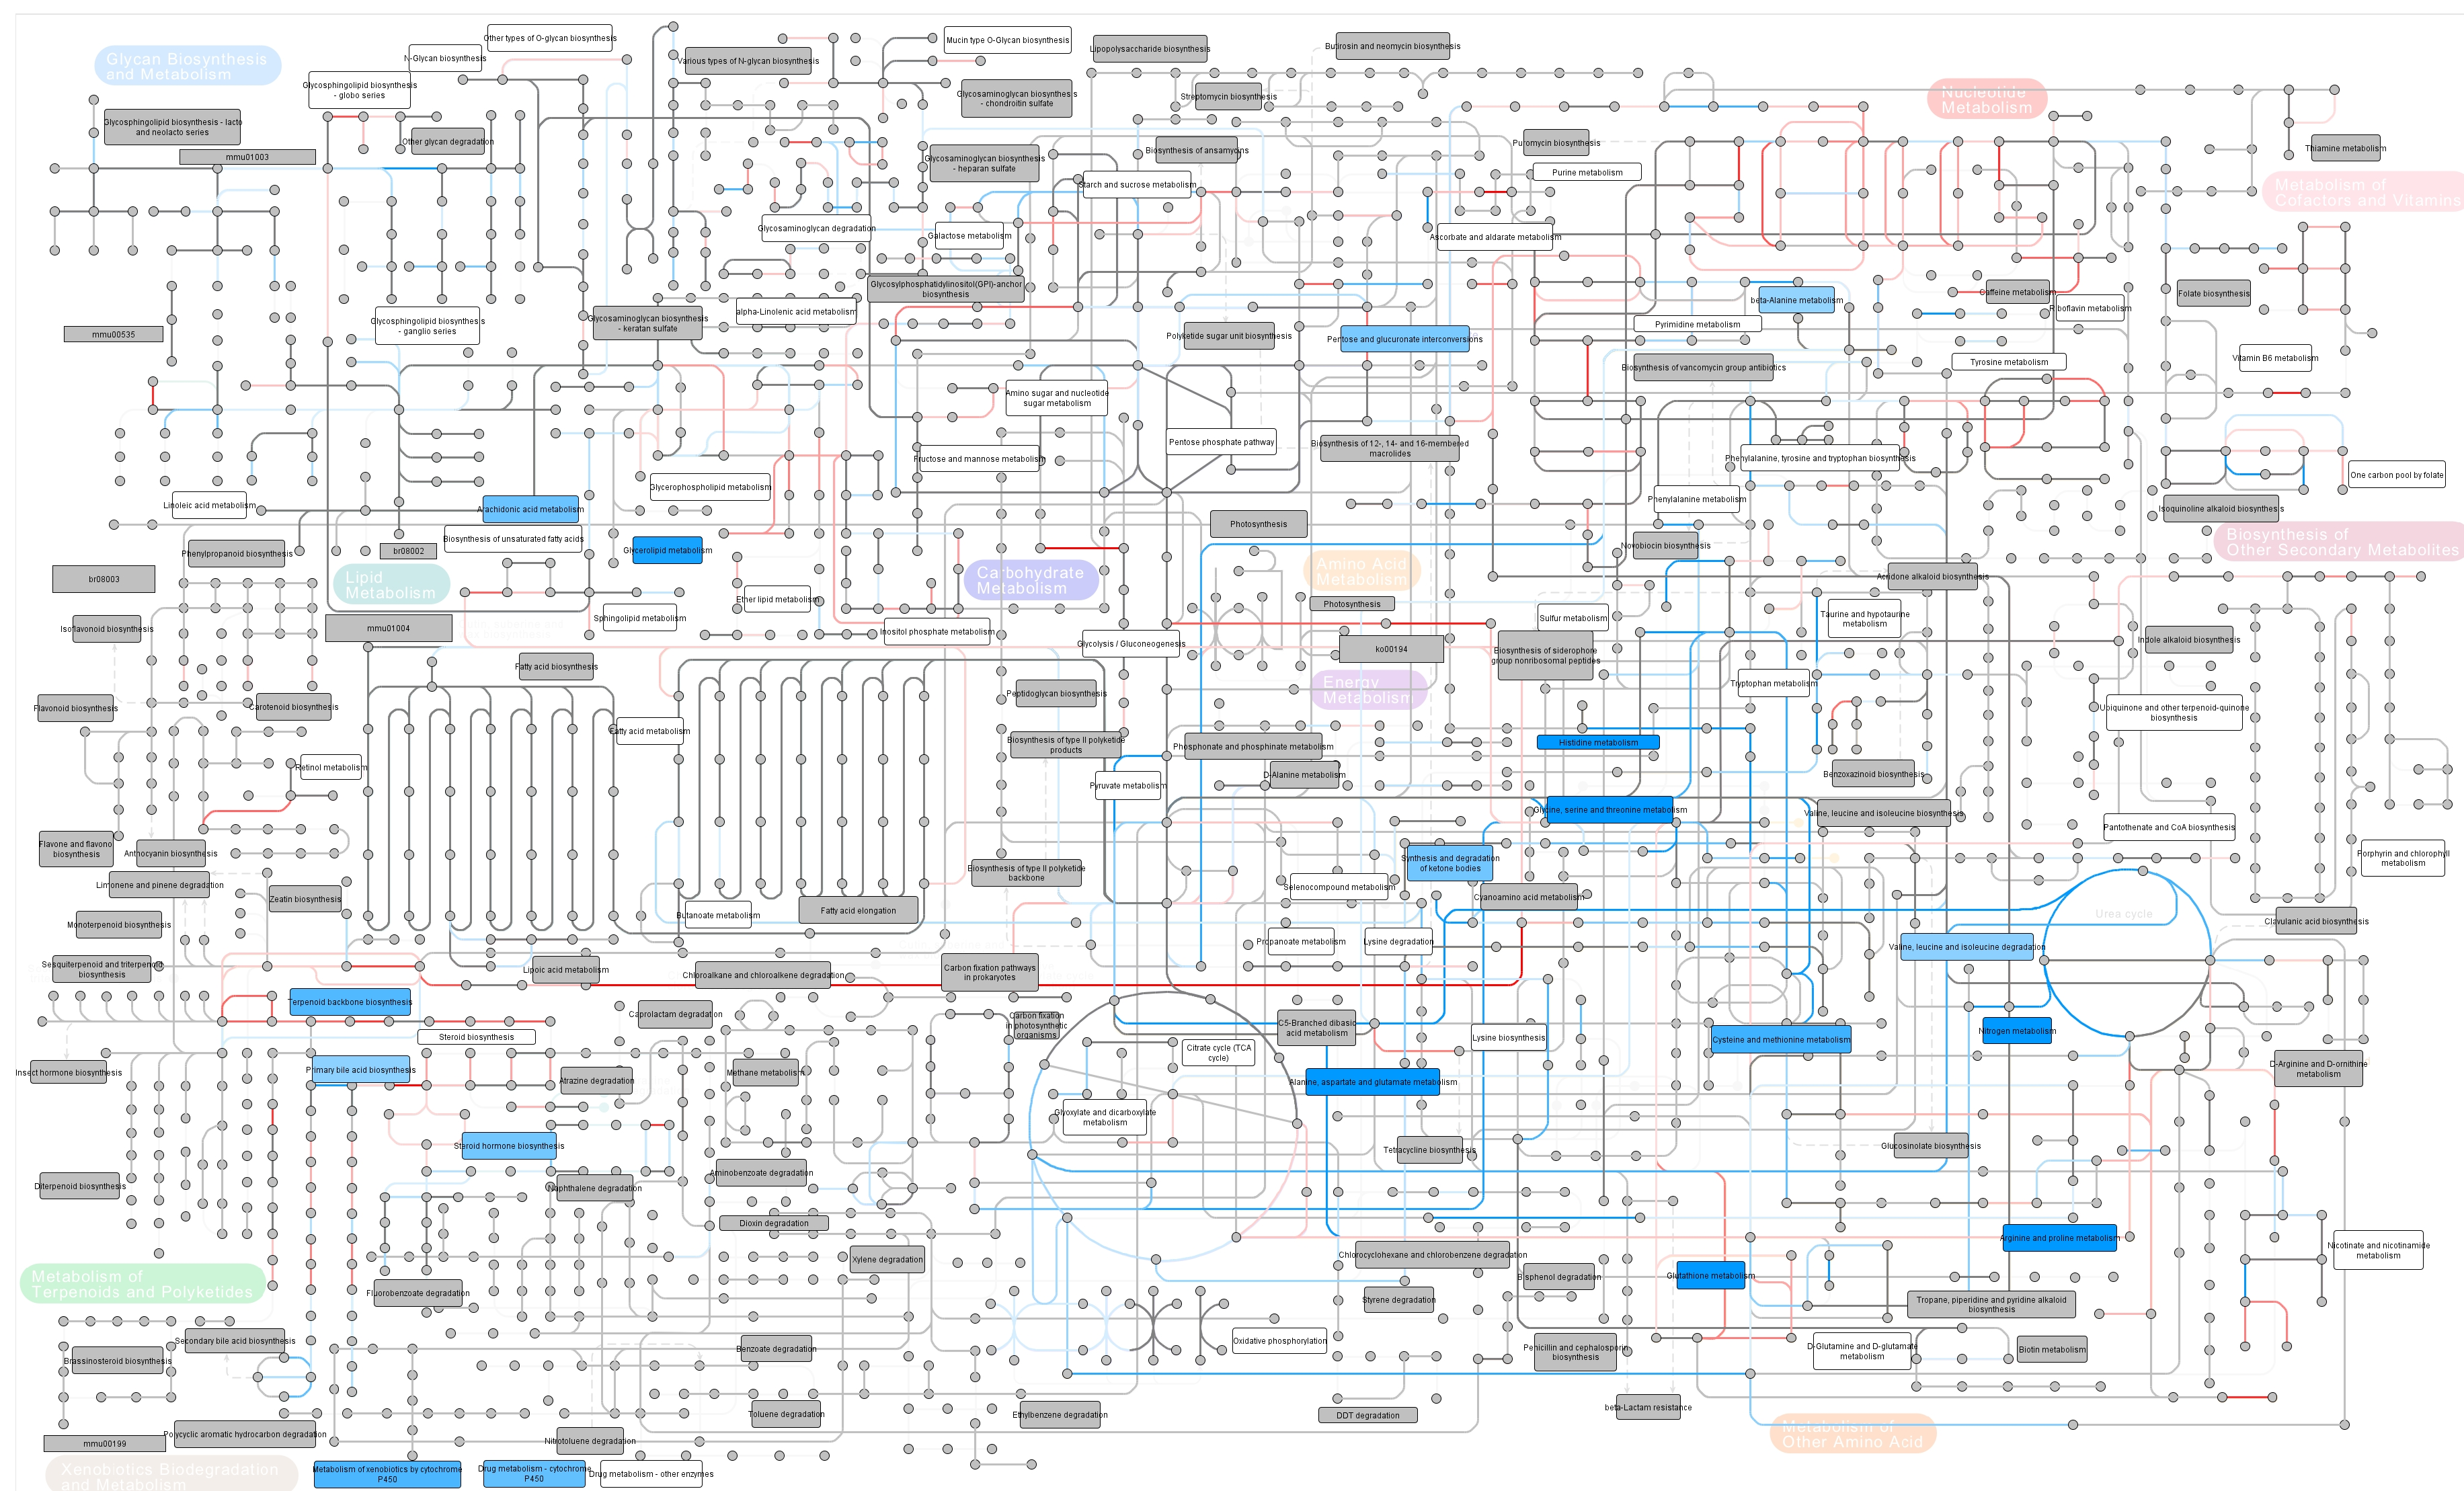
\includegraphics[width=1.0\textwidth]{figures/mmu01100_noCPDlabels.jpeg}
  \end{center}

\caption{
{\bf Comparison of an integrated and mRNA enrichment, based on data from Ctnnb1-mutated tumors.}
\TODO{Bildunterschrift, 2 Integrates a) pathway b) enrichment c) (on mRNA). 3 Can be extended to line-color mRNA 4 Volles Bild + mRNA kanten im supplement}
\TODO{\newline Was sollten wir hier genau zeigen?
\newline-- Gesamtes Bild oder bestimmter Ausschnitt? Wenn Ausschnitt, welcher?
\newline-- Kanten nach mRNA einfaerben oder nicht?
\newline-- Compound Beschriftungen verstecken oder zeigen? (Derzeit sind sie nicht beschriftet!)
}
}
\label{fig:7:metabolicOverview}
\end{figure}


%%%%%%%%%%%%%%%%%%%%%%%%%%%%%%%%%%%%%%
% Single platform in pathway visualization explanation
%%%%%%%%%%%%%%%%%%%%%%%%%%%%%%%%%%%%%%
\begin{figure}[!htb]
  \begin{center}
  %TODO: Convert to TIF (=> look at author guidelines)
    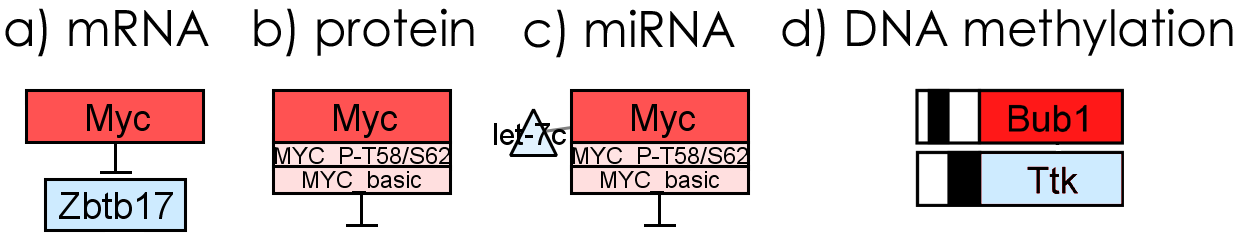
\includegraphics[width=1.0\textwidth]{figures/Platform_visualization.png}
  \end{center}

\caption{
{\bf Pathway-based visualization of different platforms.}
\TODO{Bildunterschrift}
}
\label{fig:8:pwVisPlatformsExplanation}
\end{figure}


%%%%%%%%%%%%%%%%%%%%%%%%%%%%%%%%%%%%%%
% Glycolysis mRNA/DNAm Ctnnb1/Ha-Ras Comparison
%%%%%%%%%%%%%%%%%%%%%%%%%%%%%%%%%%%%%%
\begin{figure}[!htb]
  \begin{center}
  %TODO: Convert to TIF (=> look at author guidelines)
  % Source Powerpoint file: "Glycolysis".
    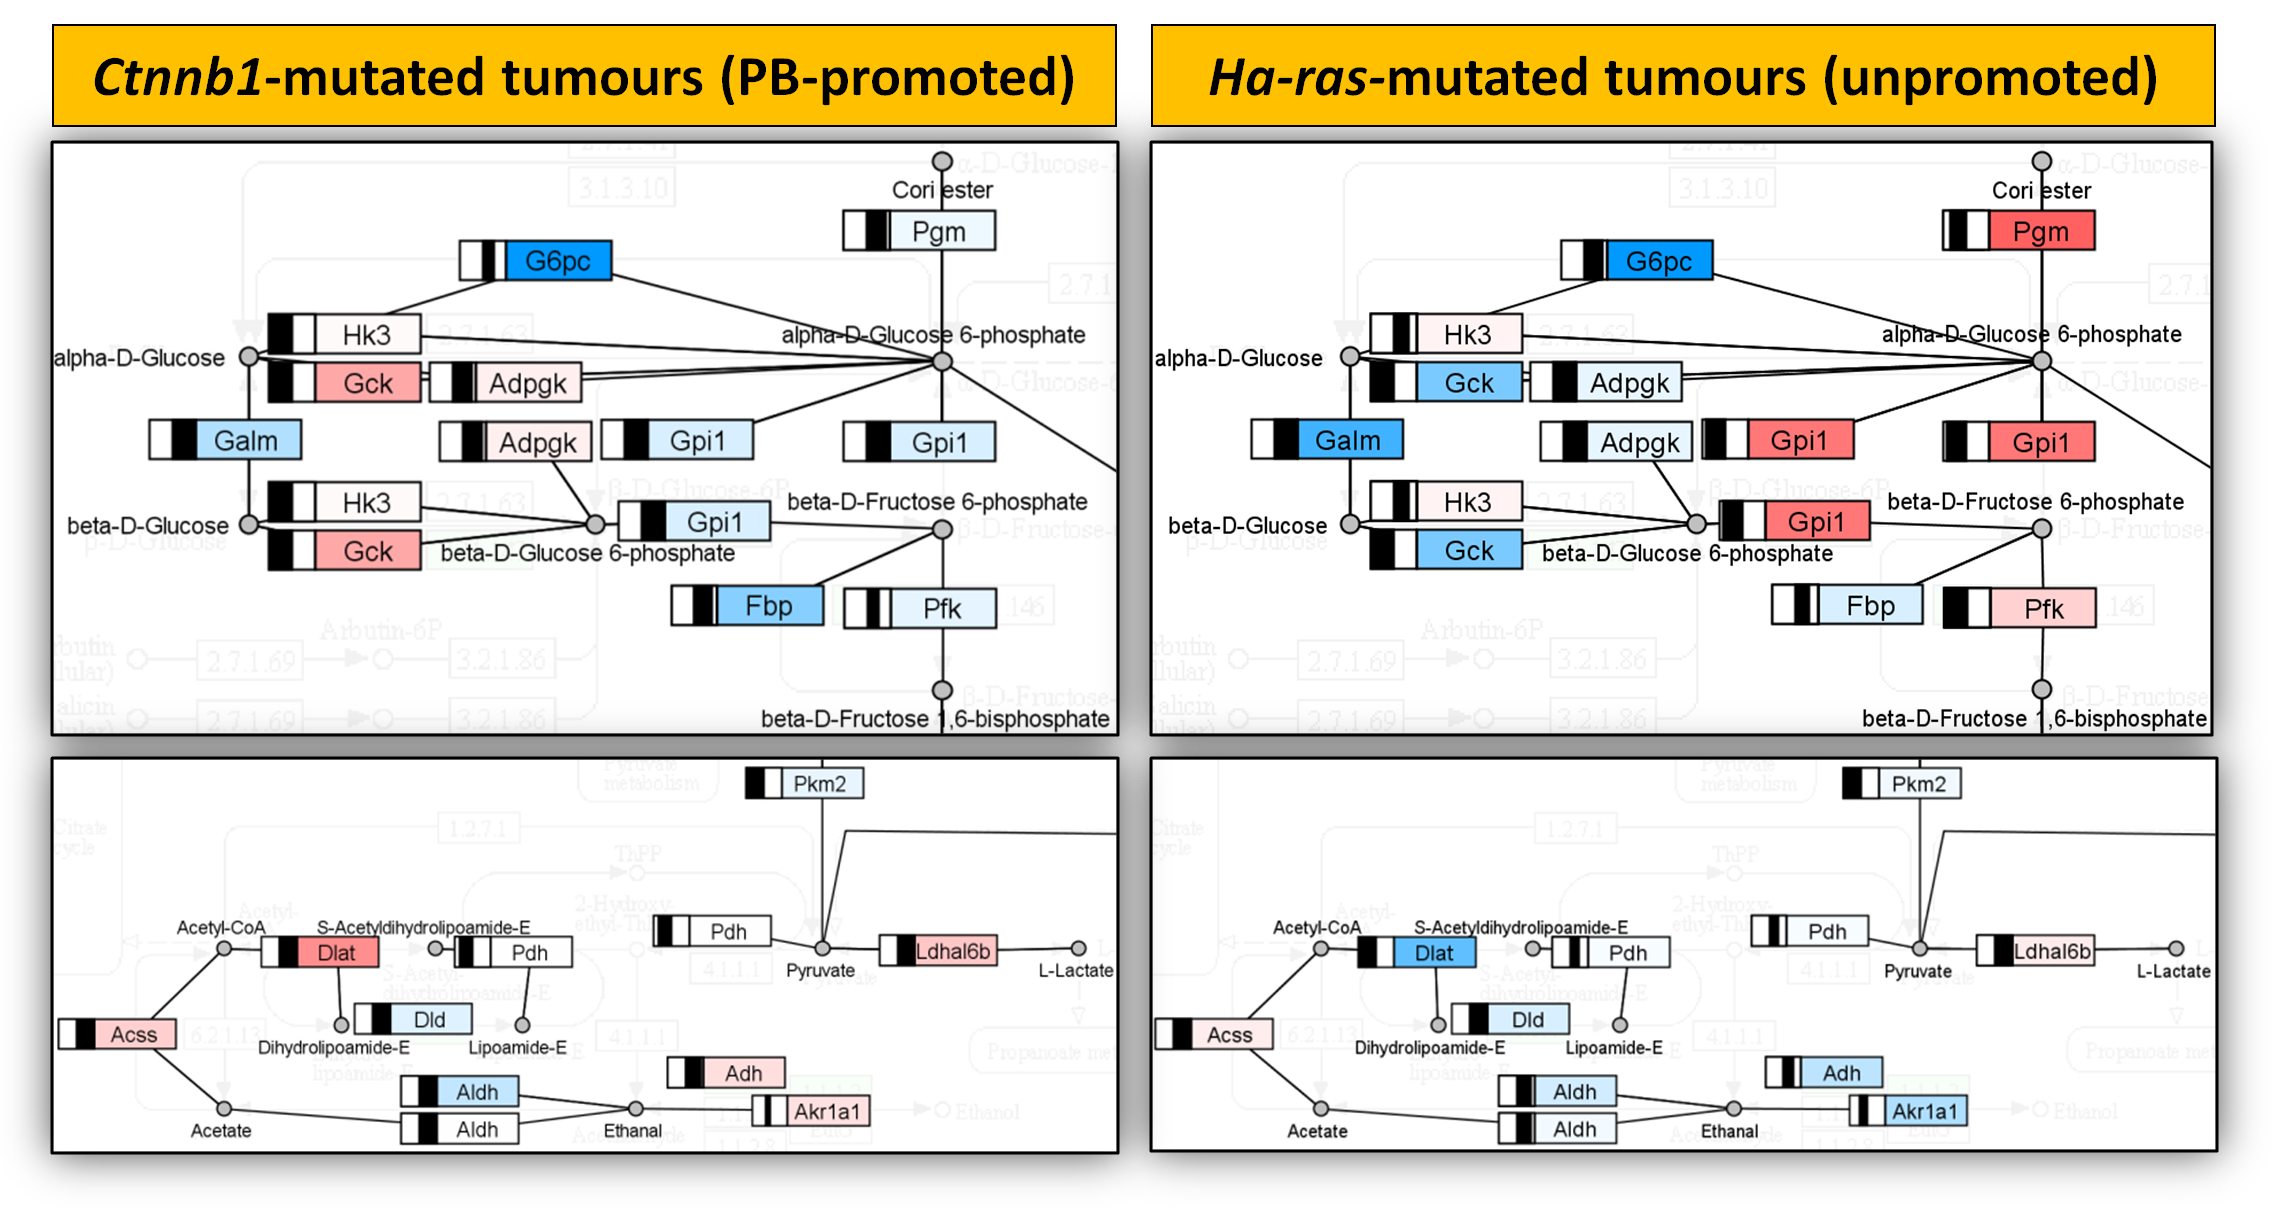
\includegraphics[width=1.0\textwidth]{figures/Glycolysis.png}
  \end{center}

\caption{
{\bf Transcriptional and epigenetic changes in Glycolysis/Gluconeogenesis during profiling of \emph{Ha-Ras} and \emph{Ctnnb1} mutated tumors.}
\TODO{Bildunterschrift, Legende (nur DNAm, mRNA)}
%
Glucokinase (Gck) -- katalysiert den 1. Schritt des Glucose-Abbaus in der Glykolyse: Genexpression hochreguliert, Promotorregion hypomethyliert.
%
Glucose-6-phosphatase (G6PC) -- katalysiert den der Gck entgegengesetzten Schritt in der Glukoneogenese, also dem Synthese von Glukose. Dieses Gen ist in beiden Tumortypen runterreguliert, dazu passt, dass die Promotorregion bei beiden weitestgehend hypermethyliert ist.
%
Fructose-1,6-bisphosphatase (FBP) -- auch ein Enzym der Gluconeogenese, in beiden Tumortypen runterreguliert mit hypermethylierter Promotorregion.
%
Bei Pgm, Aldo und anderen eingef�rbten Enzymen w�re ich pers�nlich jetzt noch vorsichtig mit irgendwelchen Aussagen, weil da oft nur sehr wenige Sonden gemessen wurden oder die Sonden widerspr�chliche Werte zeigen.
%
Korrelation von DNAm und mRNA ist teilweise recht interresant!
%
}
\label{fig:9:GlycolysisCtnnb1Ras}
\end{figure}


\section*{Tables}
%\begin{table}[!ht]
%\caption{
%\bf{Table title}}
%\begin{tabular}{|c|c|c|}
%table information
%\end{tabular}
%\begin{flushleft}Table caption
%\end{flushleft}
%\label{tab:label}
% \end{table}

\end{document}

